\documentclass{article}
\usepackage{graphicx}
\usepackage[margin=1.5cm]{geometry}
\usepackage{amsmath}
\usepackage{url}

\begin{document}

\title{Study Guide for Midterm 1: College Writing Seminar}
\author{Prof. Jordan C. Hanson}

\maketitle

\textbf{Writing is a process.}  We make a plan, create something, then stop.  The we begin to edit, delete, rearrange, until the work improves.  Eventually, it is finished.  This study guide will review the practices we've learned thus far in College Writing Seminar.  \textit{Write your responses in the same document or Google Doc.}

\section{Unit 1: Concise Writing 1}

\begin{enumerate}
\item \textit{Using the delete button} For the paragraphs below, re-write the paragraph below more concisely.  Use the following strategies: a) delete unnecessary or vague words, b) combine sentences that are about the same idea, c) make each sentence about one idea, and d) ensure a proper hierarchy of detail. \\ \\
\textbf{Create an edited version in your document.}  Biologists set out to try and record the number of fish in a lake area in order to actually better understand the wildlife populations and how it all fits together ecologically.  They get in a boat and take with them a marking paint that is also waterproof and non-toxic so that it protects the fish by not harming their scales but marks them.  Fish are lured to the boat with bait and then once they are caught, they are tagged with the paint and counted and released.  The same scientists go out to the lake area some time later, and lure fish in the same way.  Some of the fish they catch are marked and some are not.  The fraction of marked fish to the total should be true statistically of the whole population assumming the fish swim around randomly.  Thus, knowning how many fish were marked they can figure out the approximate total number of fish in the lake. \\ \\
\textbf{Create an edited version in your document.}  The mass of the Earth is $\approx 6 \times 10^{24}$ kg. It is possible to measure the mass of a black hole just like planets.  When the Earth and other planets go around the Sun, they go around it in certain orbits because of the gravitational pull between the mass of the planets and the Sun.  Using Newton's Laws of motion we can figure out the mass of the Sun if we somehow know the mass of the planets.  Astronomers observe the motion of stars around a position near the center of the Milky Way galaxy.  Stars orbit as if they are orbiting an object of extraordinary mass, a mass so large that according to general relativity it must be a black hole object.
\item \textit{Creating a map or an outline} Recall how we learned the utility of a \textit{mind map} or outline to keep our ideas organized.  Use the following lists of facts to describe how to perform the corresponding experiments.  Keep in mind that the facts are \textit{in no particular order,} so you must first organize them and then write about them. \\ \\
\textbf{Create a paragraph in your document.} 
\begin{itemize}
\item Suppose we have 100 grams of ice, and we melt it.
\item The ``latent heat of fusion'' is the heat required per mass to melt a solid substance.  For example, the latent heat for benzene is 127.40 Joules per gram.  So it would take 127.40 Joules of heat to melt 1 gram of benzene.
\item We know the heat our melter creates because we know how much power it consumes.
\item The latent heat of water is what we are trying to determine.
\end{itemize}
\textbf{Create a paragraph in your document.} 
\begin{itemize}
\item Using various cominations of LED lights in our dark room, we can create small areas with different colors of the visible spectrum.
\item Plants are evolved to photosynthesize different wavelengths of light.
\item The goal is to reveal how plant growth rate is related to the wavelength of light shining on the leaves of the plant.
\item Ten different seedlings are available.
\item We can grow the plants for one month.
\end{itemize}
\end{enumerate}

\section{Unit 2: Concise Writing 2}

\begin{enumerate}
\item \textit{Creating an outline} In class we practiced using Coggle.it to create maps of a piece of writing before writing it.  This is an important exercise, because it keeps the writing organized and the hierarchy of details intact.  \\ \\
\textbf{Create an outline or mind map} that contains the important results and landmarks in the development of the small-pox vaccine.  Helpful sources are listed below:
\begin{itemize}
\item \url{https://en.wikipedia.org/wiki/Smallpox_vaccine}
\item World Health Organization article on Smallpox vaccines
\item \url{https://www.publichealth.org/public-awareness/understanding-vaccines/vaccines-work/}
\end{itemize}
\item \textbf{Create the paragraphs in your own document.} In about 200 words, summarize the history of the development of the smallpox vaccine, and in general, how vaccination works.
\item \textbf{Create a paragraph in your own document.}  In the following example, the writing is polished but the hierarchy of details is out of order.  Re-write the paragraph so as to rearrange the details in the correct hierarchy. \\ \\

Consider a hard-boiled egg spinning on its side.  The law of conservation of momentum states that a spinning object with mass continues to spin unless a torque is applied.  Torque is an angular form of force.  The torque removes angular momentum and the egg stops.   The egg continues to spin unless it is touched, and when it is touched, the touch applies a force at some radius from the center of the egg.  Thus, when released, the raw egg yolk gives angular momentum back to the shell and the system continues to rotate.  An interesting application is to use this experiment to determine if an egg is hard-boiled.  Touching a spinning raw egg only removes the angular momentum of the shell, and the yolk continues to spin inside.  A hard-boiled egg stops and remains motionless.
\end{enumerate}

\section{Unit 3: Technical Description 1}

\begin{enumerate}
\item \textit{Removing ambiguous words}  In the following sentences, remove the ambiguous words, and either replace them with quantifiable concepts, or simply cut them. \\ \\
\textbf{Write the new sentences in your own document.} 
\begin{itemize}
\item The pod of dolphins was pretty large, as surfacing individuals could be seen for hundreds of yards.
\item The age of the coral reef was very old, and many different species had evolved to live within it.
\item The polar vortex weather front will arrive soon, and bring with it record low temperatures.
\item A marathon runner ran the full 42.2 km of the race in 2.5 hours, making his average speed fairly quick.
\end{itemize}
\item \textit{Spatial detail, perspective}  \\ \\
\textbf{Write a paragraph in your own document.}  Repeat the exercise we performed in class, in which you described precisely how to find an item on your desk, starting from the front door. Instead, imagine you are either a) at work, or b) at your old high school.  Starting from the main entrance, describe exactly how to travel from the main entrance to your favorite spot.  Pay special attention to the perspective of the reader: are you carrying the reader's perspective with each step?
\item \textit{Temporal detail, perspective in time} \\ \\
\textbf{Write a paragraph in your own document.}  Repeat the exercise we performed in class in which we wrote down from memory our favorite recipe step by step.  Instead of simply our favorite recipe, choose from the following list of topics:
\begin{itemize}
\item How to change a car tire
\item How to build a treehouse
\item How to walk a dog in your neighborhood
\item How to perform your athletic exercise or training routine
\item How to hike your favorite trail
\end{itemize}
Pay special attention to the temporal order of details, and the temporal perspective of the reader.  Are you picking up the reader's temporal perspective and moving it through time?
\item \textit{Dispassionate description} \\ \\
\textbf{Write two to three sentences in your own document.}  Recall the exercise we performed in class, in which we described an image objectively, without using language shaded with our own interpretation of what is happening in the image.  Use this technique on the image in Fig. \ref{fig:caravan}.

\begin{figure}
\centering
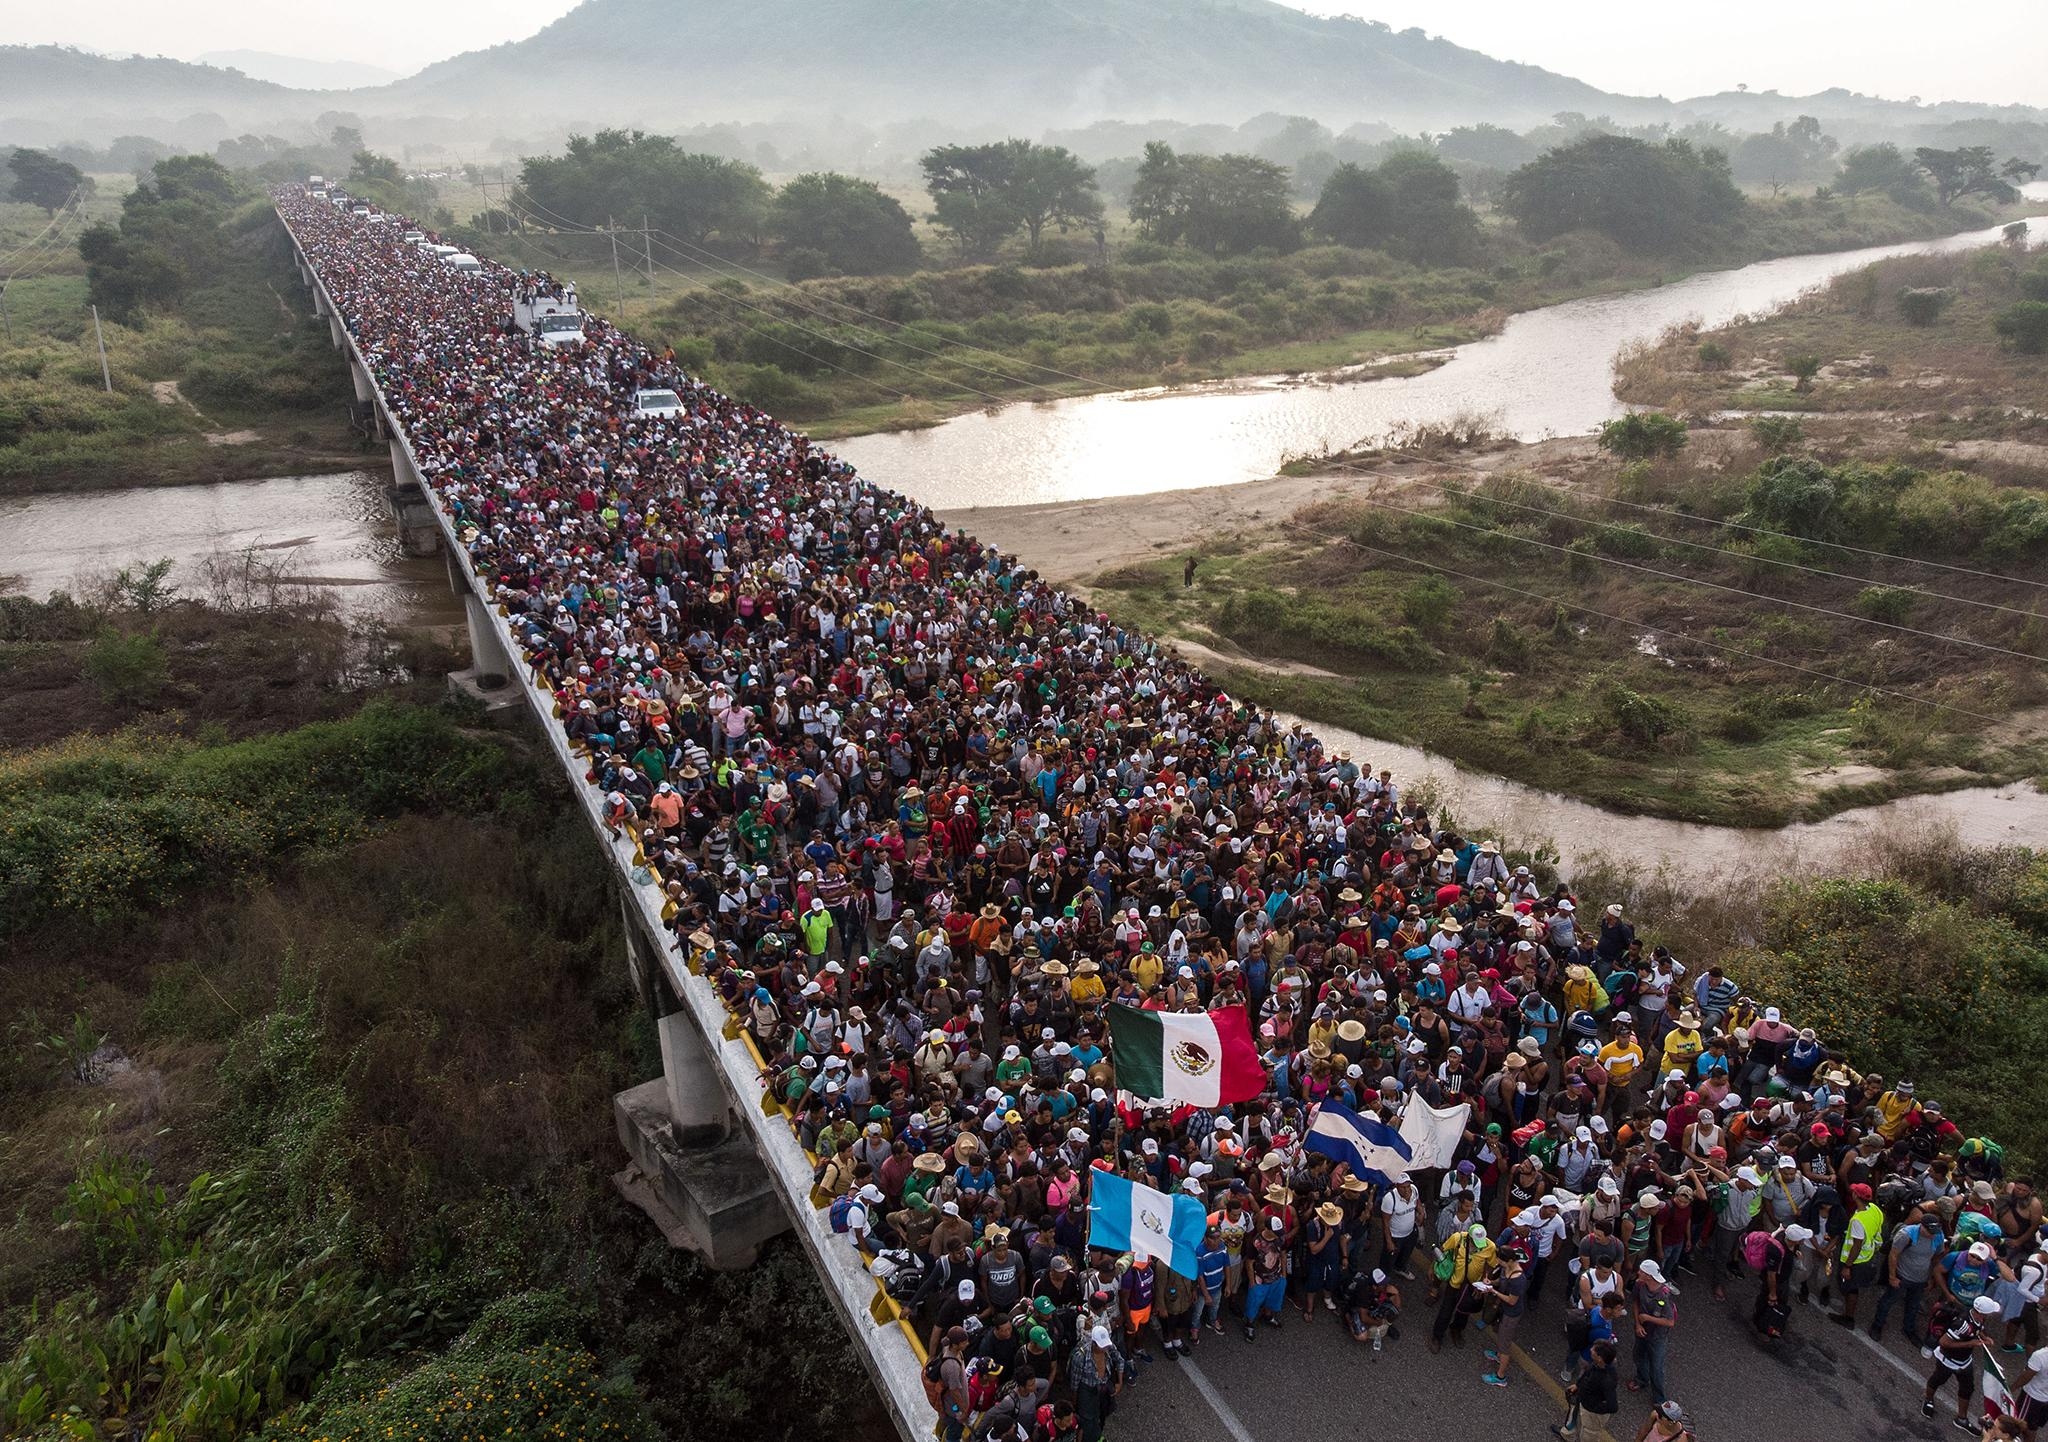
\includegraphics[width=7cm]{figures/caravan.jpg}
\caption{\label{fig:caravan} Describe this photo with objective language.}
\end{figure}
\end{enumerate}

\section{Unit 4: Technical Description 2}

\begin{enumerate}
\item \textit{Using passive voice and past tense} In technical and scientific writing, first person and present tense are rarely used.  Instead, we mostly convert to passive voice and third person.  For example, \\ \\
I am measuring the specific heat of the liquid by adding a fixed amount of heat per unit time to a sample of it, and plotting the heat added versus temperature.  The slope of this line divided by the mass of the liquid is the specific heat. \\ \\
\textit{This becomes:} The specific heat of the liquid was measured by adding a fixed amount of heat per unit time to a sample with known mass.  The heat added was plotted versus the change in temperature.  The slope of this line, divided by the mass, was calculated.  The result was the specific heat. \\ \\
\item \textit{Convert the following paragraph into passive third person.}
\begin{quote}
We sent our survey in 2020 to 1350 young adults, which asked them about their mental health status.  Two years later we sent the same survey to the same 1350 young adults.  In 2022, these young adults are seniors in high school.  We asked them the following questions: (1) Has your mental health improved or not improved since 2020? (2) Did the pandemic and remote learning impede your educational progress in mathematics? (3) Do you plan to enter a profession focused on the use of mathematics?  We analyzed the data and found a correlation between mental health issues and the educational impact of the pandemic.  The correlation corresponds to a p-value of 0.04, but we discuss also the size of the effect and the next steps to take.
\end{quote}
\end{enumerate}

\end{document}